
\section{Additional Details}
%
\paragraph{Broader impact}
%
FDMs are widely used in the context of learning to predict the evolution of dynamical systems. The model class presented in this work, \ourmethod{}, provides an accessible way to train and evaluate large-scale FDMs, reducing memory overhead and overall training times. When predicting the solution of e.g. a \textit{partial differential equation} (PDE), care should be taken especially when the prediction is used to inform downstream decision making, as many systems are optimally predictable only for a certain time scale \citep[pp. 366]{strogatz2018nonlinear}. We anticipate a potential positive environmental impact from the adoption of \ourmethod{} as a replacement for the largest FDMs currently in use. 
%

\paragraph{Experimental setup} Experiments have been performed on an \textsc{NVIDIA\copyright~DGX} workstation equipped with a 128 threads \textsc{AMD\copyright~Epyc 7742} CPU, 512GB of RAM and four \textsc{NVIDIA\copyright~A100} GPUs. The main software implementation has been done within the $\tt PyTorch$ \citep{paszke2017automatic} ecosystem building upon the $\tt pytorch$-$\tt lightning$ \citep{falcon2019pytorch} framework. 
%

\paragraph{Common experimental settings} 
%
\subsection{Incompressible Navier–Stokes}\label{asec:exp_nvs}
%
\paragraph{Dataset}
%
We use data generated in \citep{li2020fourier} in the form of pairs of initial conditions and solutions of the incompressible Navier-Stokes equations in vorticity form solved with a pseudospectral method. The dataset \footnote{Data can be downloaded here: \href{https://drive.google.com/drive/folders/1UnbQh2WWc6knEHbLn-ZaXrKUZhp7pjt-}{Google Drive link}. High viscosity: {\tt NavierStokes\_V1e-3\_N5000\_T50}, Low viscosity: {\tt NavierStokes\_V1e-4\_N10000\_T30}.} is comprised rollouts of solutions as images of resolution $64$.

\paragraph{Models and training}
%
The training configuration is shared by all models:

\begin{listing}[H]
\begin{mintedbox}{yaml}
datamodule: 
    ntrain: 1000
    ntest: 200
    batch_size: 64
    history_size: 1
train:
    optimizer: 
        type: AdamW
        learning_rate: 1e-3
        weight_decay: 1e-4
    scheduler: 
        type: Step
        step_size: 100
        gamma: 0.5
        scheduler_interval: epoch
loss_fn: RelativeL2Loss
\end{mintedbox}
\vspace{-6mm}
\end{listing}
%
For the high viscosity ($1e^{-3}$) setting, the models are trained to predict the solution at time $T=50$ seconds directly, without producing rollouts and supervising the model with solutions at times between $0$ and $50$. Crucially, this ensures that the task is much more challenging than that of \citep{li2020fourier}, where for a single training sample the entire rollout is used as supervision. For the low viscosity setting ($1e^{-4}$), target times are $T=15$ seconds.

Model configurations are given below:

\begin{listing}[H]
\begin{minipage}[t]{0.32\textwidth}
\begin{mintedbox}{yaml, title=\config{FNO}}
FNO:
    modes: 24
    nlayers: 6
    width: 32 \end{mintedbox}
\end{minipage}
%
\begin{minipage}[t]{0.32\textwidth}
\begin{mintedbox}{yaml, title=\config{\ourmethod{}}}
T1:
    modes: 24
    nlayers: 6
    width: 48  \end{mintedbox}
\end{minipage}
%
\begin{minipage}[t]{0.32\textwidth}
\begin{mintedbox}{yaml, title=\config{FFNO}}
FFNO:
    modes: 32
    nlayers: 10
    width: 82 \end{mintedbox}
\end{minipage}
\vspace{-6mm}
\end{listing}

where each layer in a model shares the same structure. In FNOs and FFNOs, we employ a regular FDM layer following \citep{li2020fourier,tran2021factorized} with k-space convolutions and residual connections given by n-space layers (pointwise convolutions for FNOs, dense for FFNOs). \ourmethod{} uses a similar layer without n-space residual paths. The differences in number of layers and width have been introduced to keep parameter counts comparable. At a given channel width, FNOs require the largest number of parameters due to k-space convolutions on complex numbers given by the DFT coefficients. Although FFNOs \citep{tran2021factorized} are most parameter efficient due to parameter sharing, we found them unable to tackle the task and produce high-quality predictions.  

\begin{figure*}[h!]
    \centering
    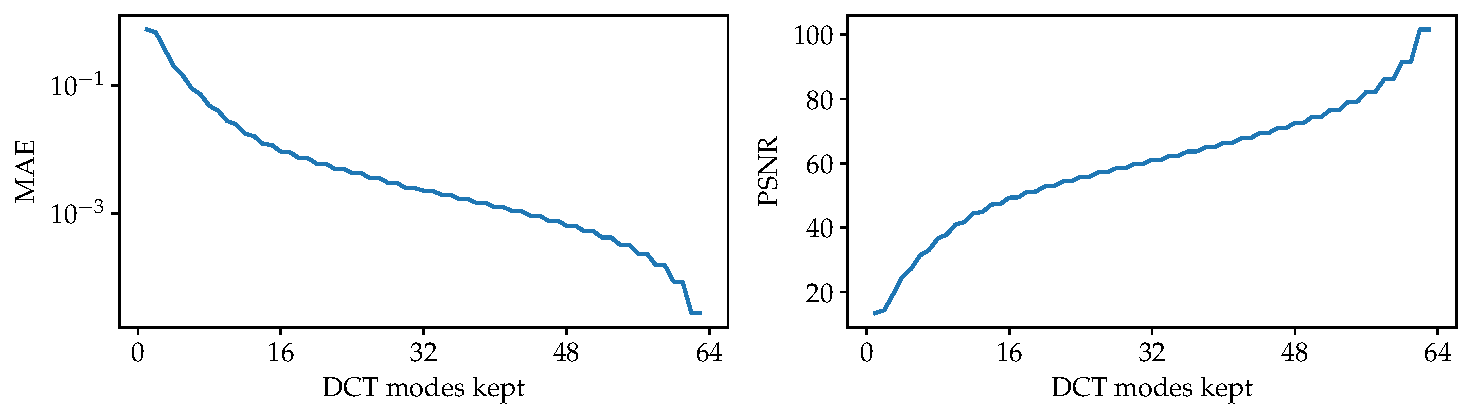
\includegraphics[width=0.8\linewidth]{figures/navier_stokes_error_vs_dct_modes.pdf}
    \vspace{-3mm}
    \caption{\small Incompressible Navier-Stokes: metrics vs number of DCT modes (i.e. $m$ elements) kept (i.e. not pruned).}
    \label{fig:navier-stokes-modes-mae-psnr}
\end{figure*}



\ourmethod{+} employs a UNet on the patch constructed by the elements of the k-space kept, and shares its structure with \ourmethod{} otherwise. The {\tt vp} parameter initialization scheme in \ourmethod{} is applied only to the first layer performing the truncation in k-space, not to the following layers which use standard Kaiming initialization \cite{he2015delving}. In FNOvp the scheme is applied to all layers.


\begin{figure*}[h!]
    \centering
    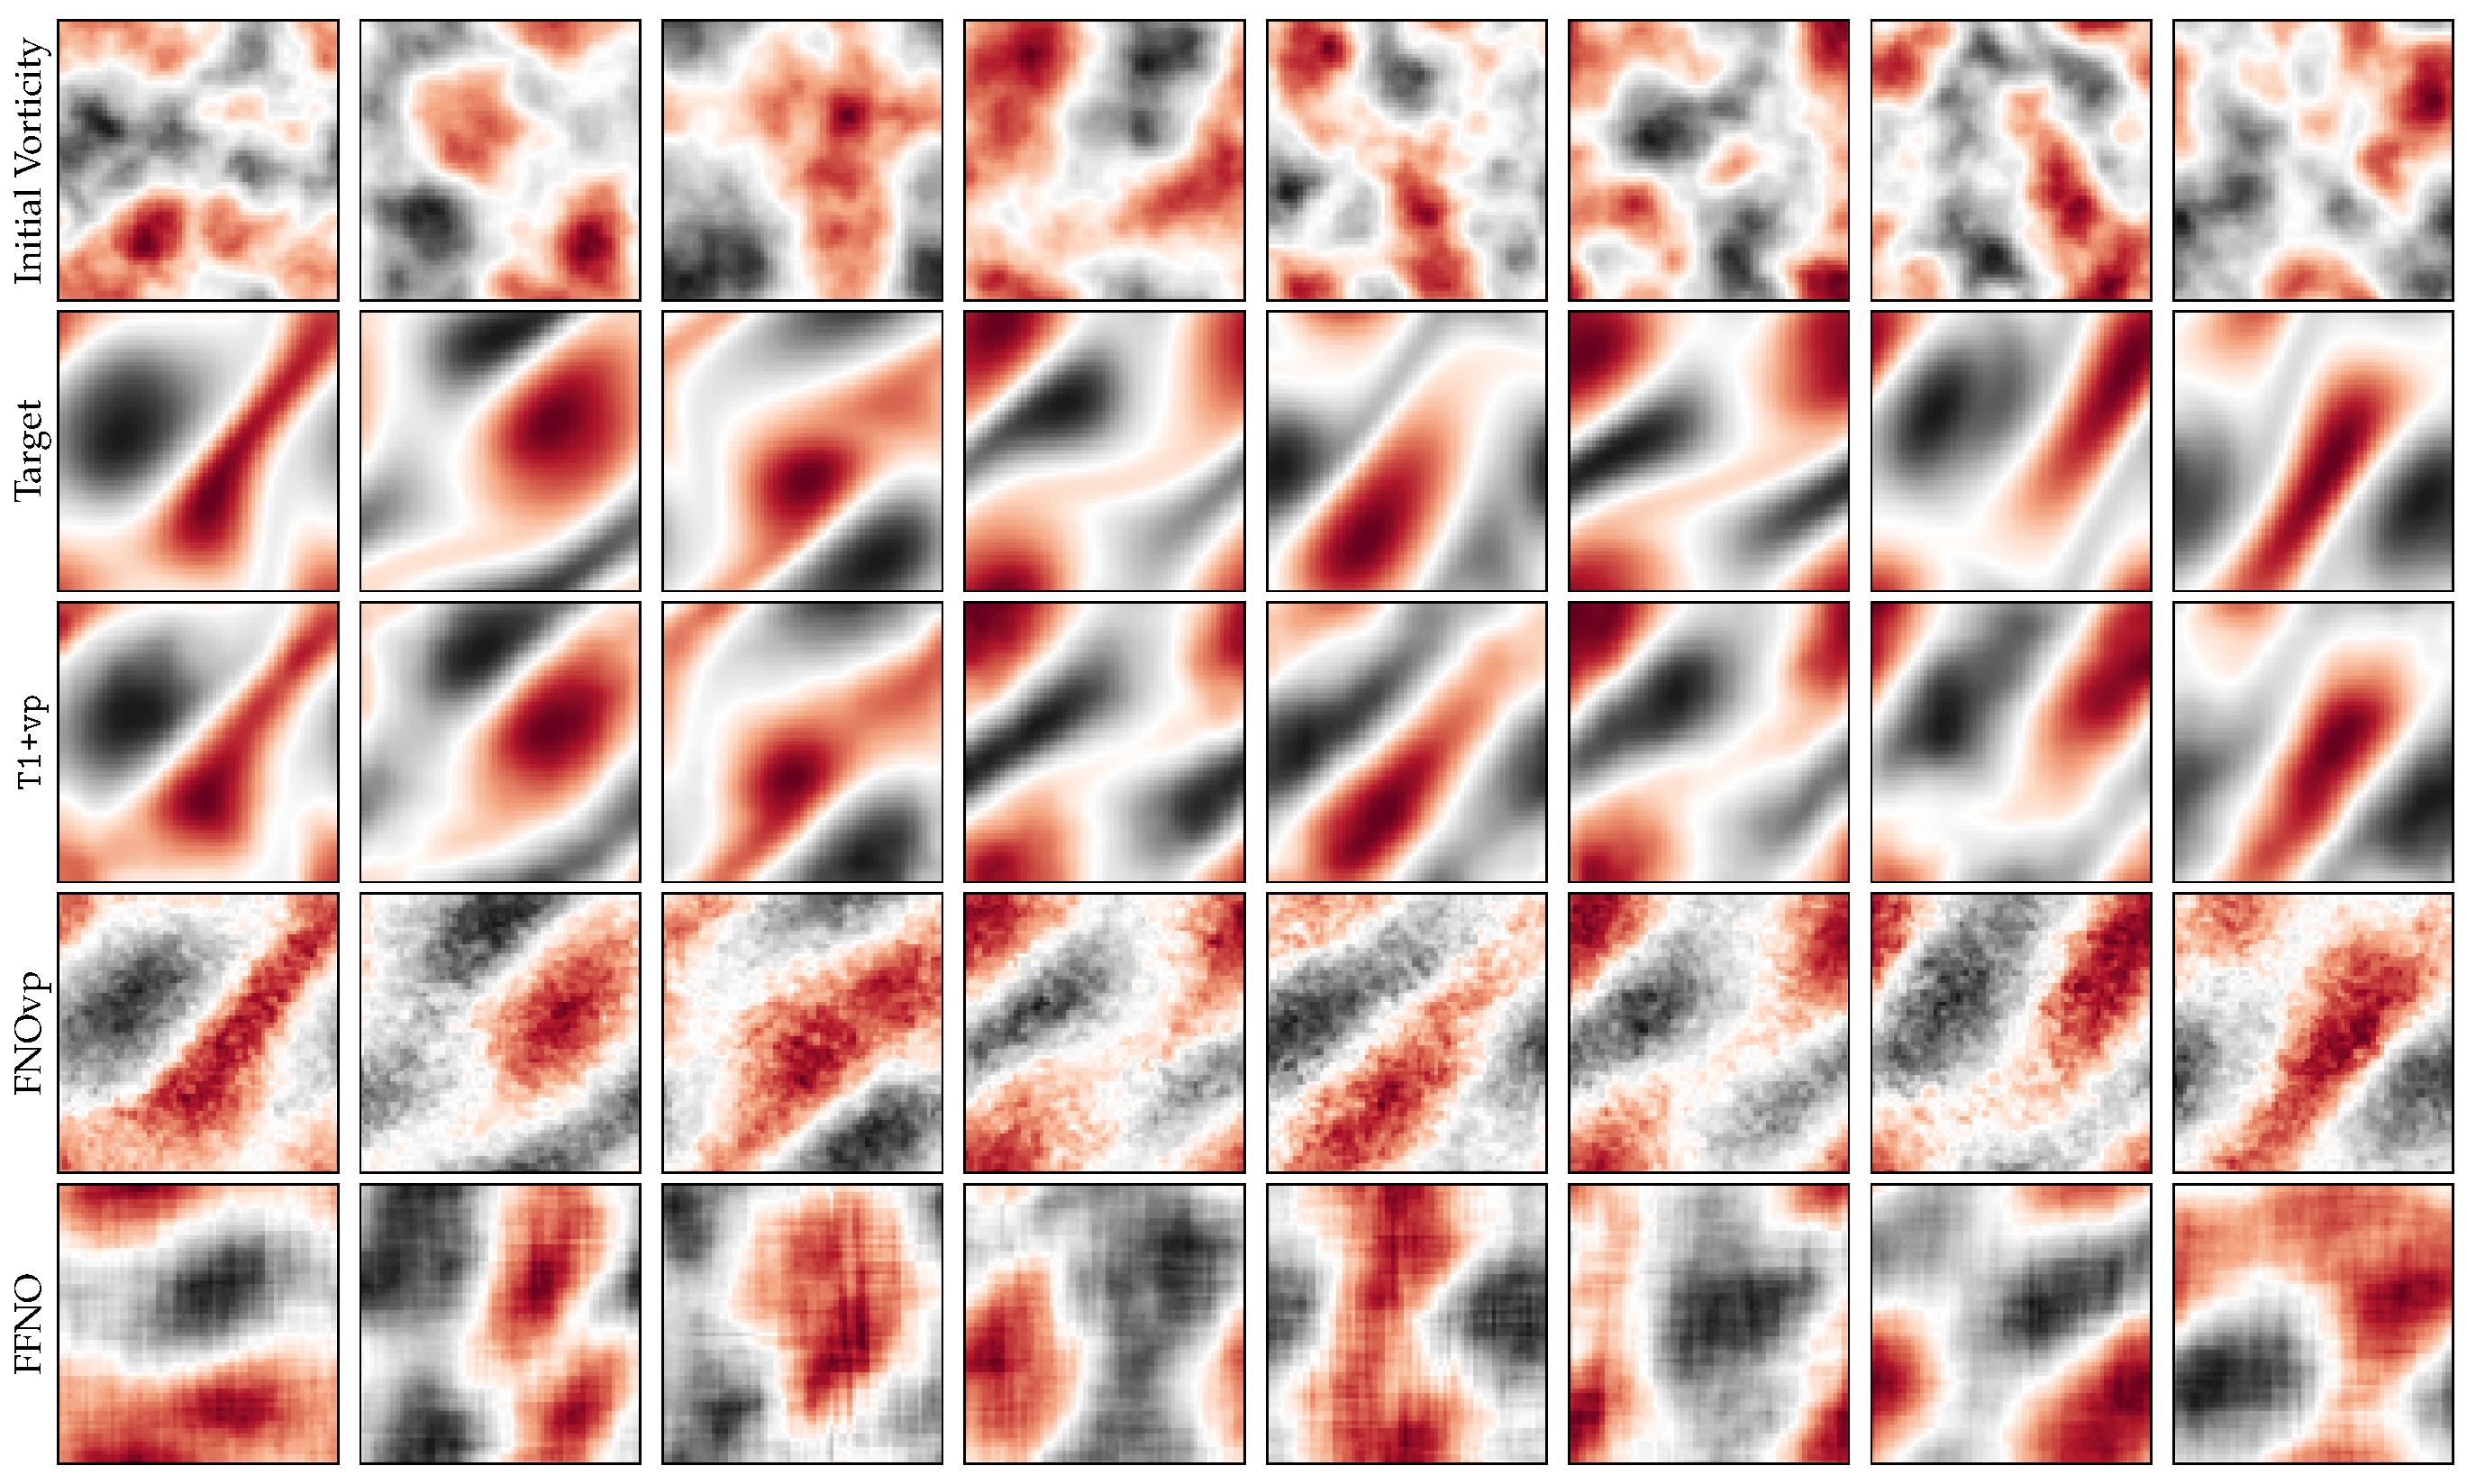
\includegraphics[width=\linewidth]{figures/navier_stokes_predictions_big.pdf}
    \vspace{-3mm}
    \captionof{figure}{\small Initial conditions, ground truth solutions at time $T=50$ seconds, and models predictions for incompressible Navier-Stokes in vorticity form (high viscosity of $1e^{-3}$). \ourmethod{} reduces solution error w.r.t FNOs by over $20\%$ and FFNOs by over $40\%$. A single forward pass of \ourmethod{} models is on average $2 \times$ faster than FNO and $10\times$ than FFNOs. }
\label{fig:navier-stokes-predictions-big}
\end{figure*}

\paragraph{Hyperparameter tuning}
%
We start with the basic model structure of FNOs as detailed \citep{li2020fourier} and perform a basic hyperparameter search on a small slice of the training set, with the goal of ensuring proper convergence of a model. We did not find the number of layers to have a significant impact on convergence. Width plays an important role and is best kept above $24$.

%
\paragraph{Scaling laws}
%
We use the same settings as the main experiment, repeating separate training runs for the low viscosity setting. In particular, we increase the dataset size for each set of runs by a factor of $2$: $1024, 2048, 4096, 8192$. The total number of epochs is kept fixed, so that more iterations are performed for larger datasets. The same test set of size $200$ is used in all cases.
%

\paragraph{Further comments}
Additional predictions are provided in \cref{fig:navier-stokes-predictions-big}. \cref{fig:navier-stokes-modes-mae-psnr} shows the approximation error on the Navier-Stokes solutions due to truncation at different number of k-space elements $m$.


\subsection{Flow Around Airfoils}\label{asec:exp_dfp}
%
\paragraph{Dataset}
%
We use a slice of the dataset introduced by \cite{thuerey2020deep} in the form of $11000$ training pairs of initial conditions and solutions. The solutions are obtained via {\tt OpenFOAM} \citep{jasak2007openfoam} SIMPLE, a steady-state solver for incompressible and turbulent flows. In particular, the initial conditions are specified as freestream velocities over the domain (two-directional components), in addition to a specification of the airfoil in point cloud format. Delaunay triangulation is used for mesh generation.

After simulation, data is provided as initial condition and steady-state solution pairs. The initial condition is a three channel $128 \times 128$ image: two channels for freestream velocities and one for the airfoil mask. The solution is a three channel $128 \times 128$ image: a velocity field and a scalar pressure field. All data is normalized using training set statistics.
%

\paragraph{Models and training}
%
Training configuration is given as

\begin{listing}[H]
\begin{mintedbox}{yaml}
datamodule: 
    ntrain: 8000
    nval: 2000
    ntest: 1000
    batch_size: 64
train:
    optimizer: 
        type: AdamW
        learning_rate: 1e-3
        weight_decay: 1e-4
    scheduler: 
        type: Step
        step_size: 100
        gamma: 0.6
        scheduler_interval: epoch
loss_fn: RelativeL2Loss
\end{mintedbox}
\vspace{-6mm}
\end{listing}

The baseline UNet matches the architecture of \citep{thuerey2020deep} (DFPNet). The FNO architecture is comprised of a standard stack of FDM layer as discussed in \ref{asec:exp_nvs}. The k-space UNet in \ourmethod{+} has the same structure as a DFPNet.

\begin{listing}[H]
\begin{minipage}[t]{0.32\textwidth}
\begin{mintedbox}{yaml, title=\config{FNO}}
FNO:
modes: 24 
nlayers: 6
width: 48  \end{mintedbox}
\end{minipage}
%
\begin{minipage}[t]{0.32\textwidth}
\begin{mintedbox}{yaml, title=\config{DFPNET}}
DFPNET:
channel_exponent: 6 \end{mintedbox}
\end{minipage}
%
\begin{minipage}[t]{0.32\textwidth}
\begin{mintedbox}{yaml, title=\config{\ourmethod{+}}}
T1+: 
modes: 100 
channel_exponent: 5 \end{mintedbox}
\end{minipage}
\vspace{-6mm}
\end{listing}

\begin{figure*}[h!]
    \centering
    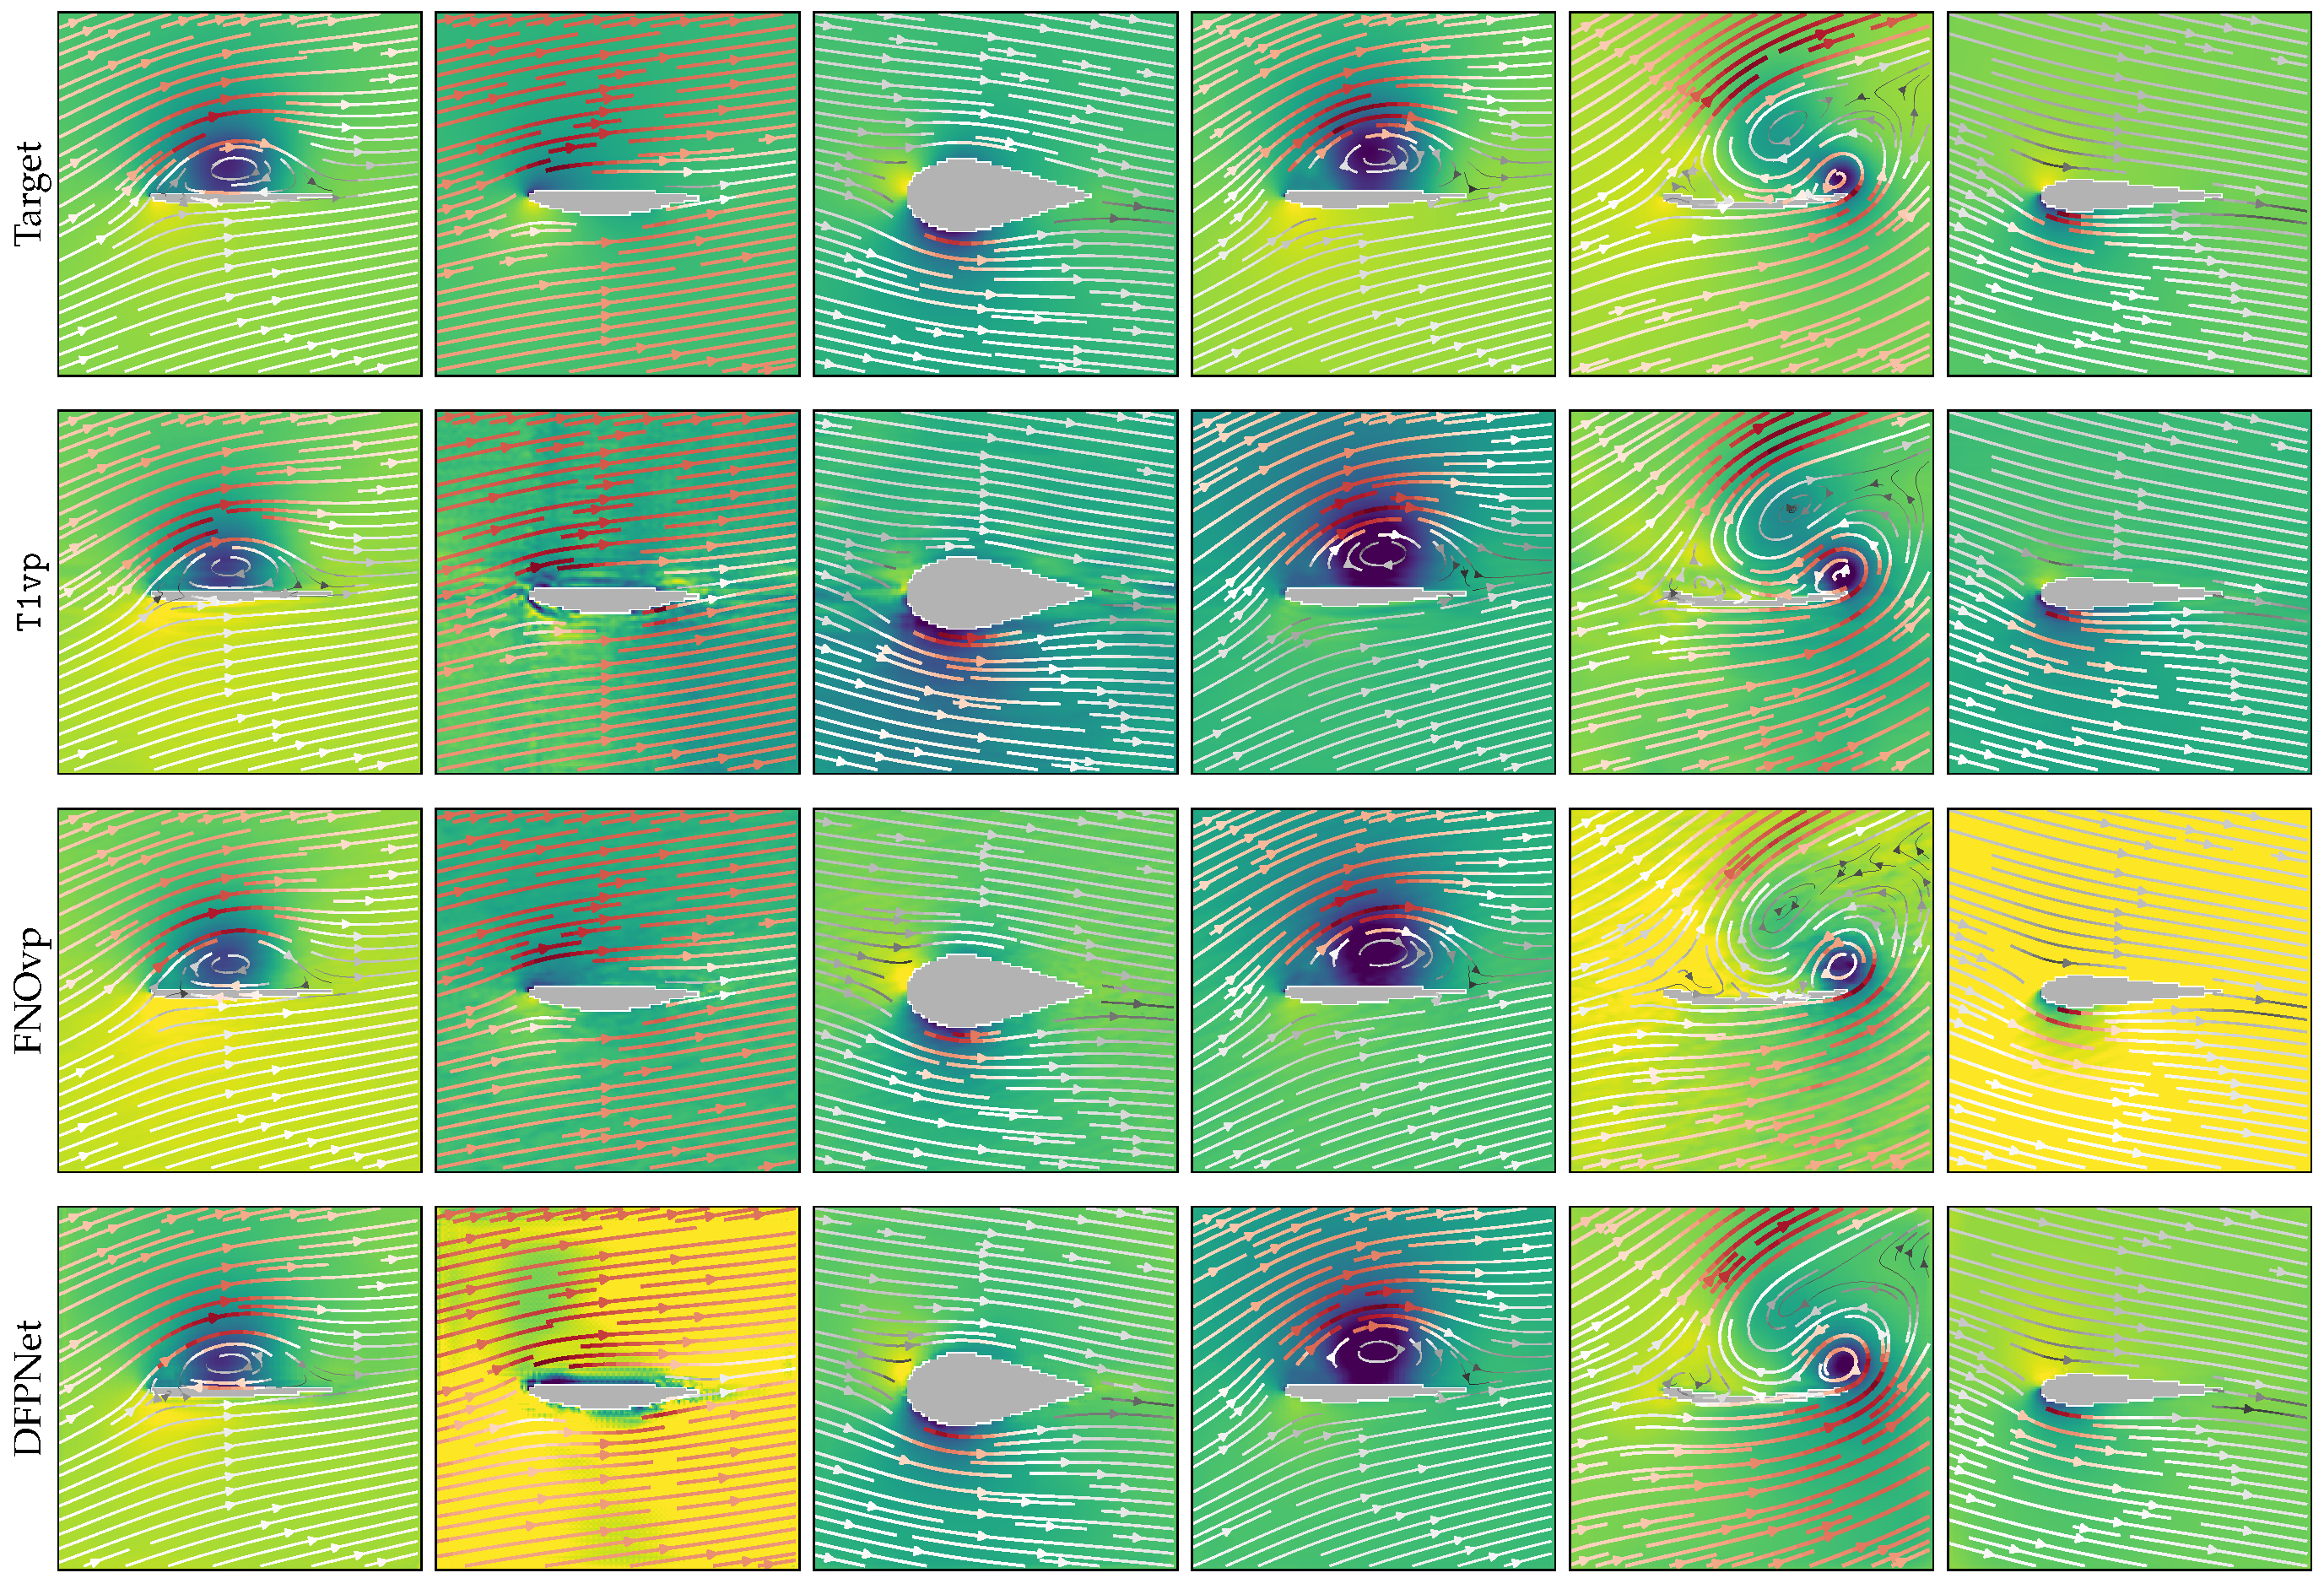
\includegraphics[width=\linewidth]{figures/dfp_predictions_big.pdf}
    \vspace{-4mm}
    \captionof{figure}{\small Ground truth solutions and predictions with different airfoil designs and angles of attack of the flow. The background color is the scalar pressure value while the vector field represents the velocity field: arrow colors indicate its "strength" i.e. $2$-norm.}
\label{fig:dfp-predictions-big}
\end{figure*}

\begin{figure*}[h!]
    \centering
    % \vspace{-10mm}
    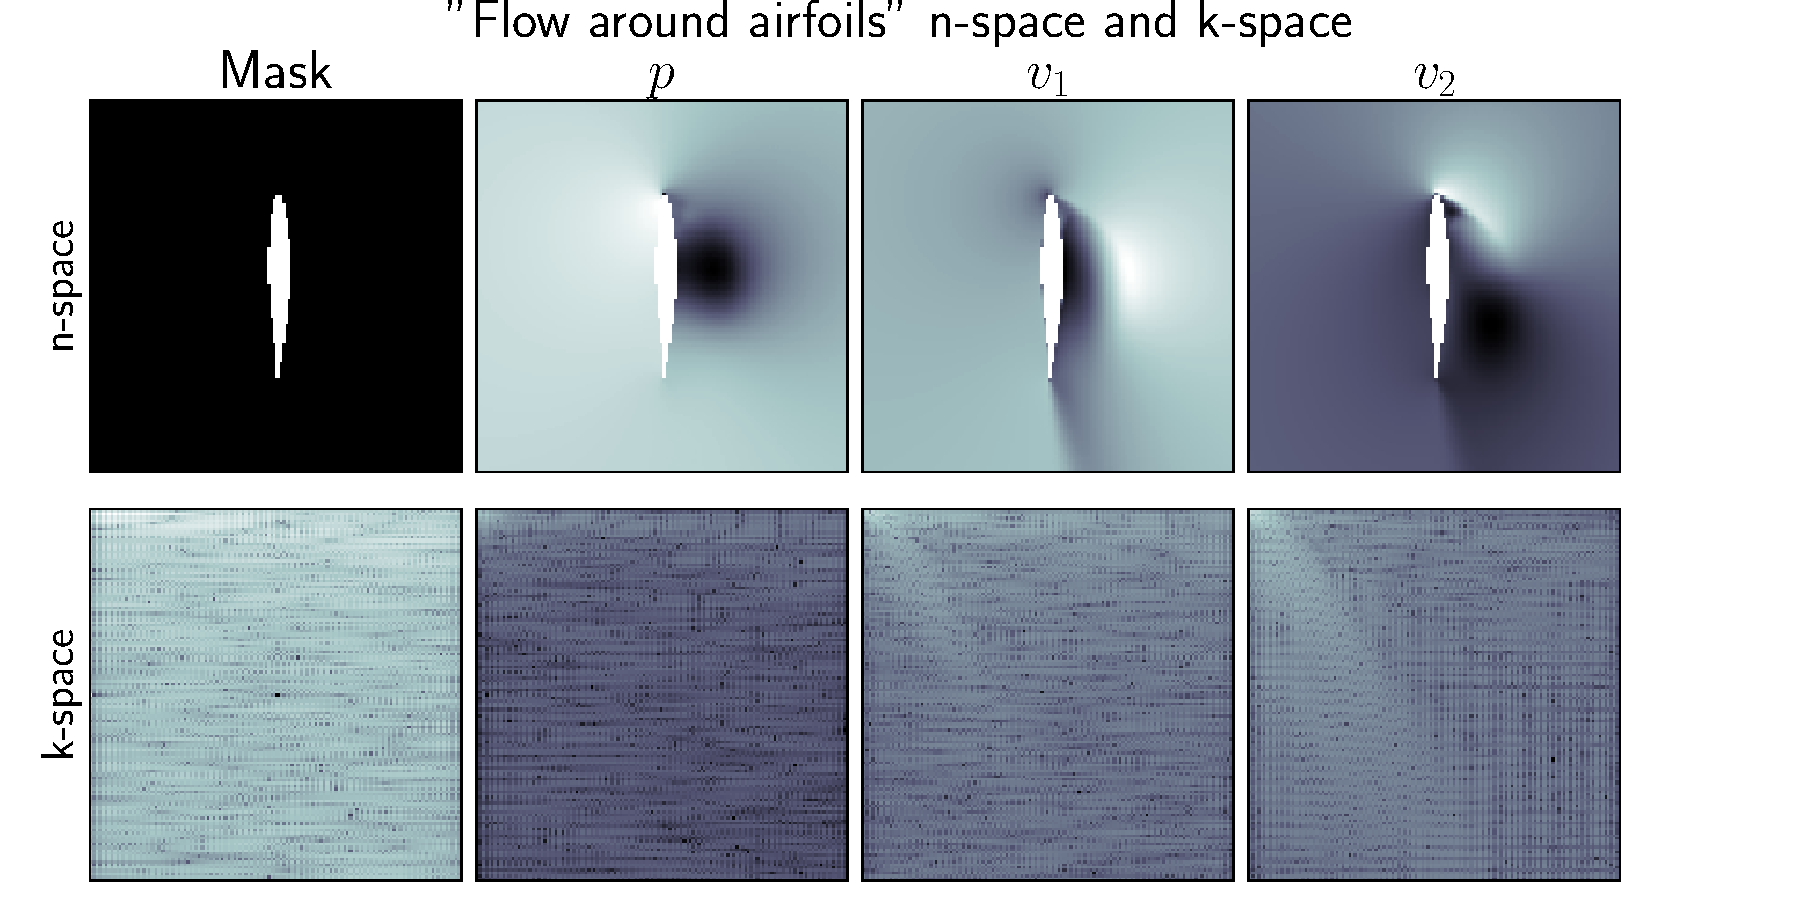
\includegraphics[width=0.75\linewidth]{figures/dfp_kspace.pdf}
    % \vspace{-3mm}
    \vspace{-3mm}
    \caption{\small Flow around airfoils: example of n-space: input mask, output pressure $p$ and velocity field $v_1, v_2$. Below, the corresponding DCT k-space in abs-log i.e. $\log{(|\cT(x)|)}$ to highlight its structure.}
    \label{fig:dfp-nspace-kspace}
\end{figure*}

\begin{figure*}[h!]
    \centering
    % \vspace{-10mm}
    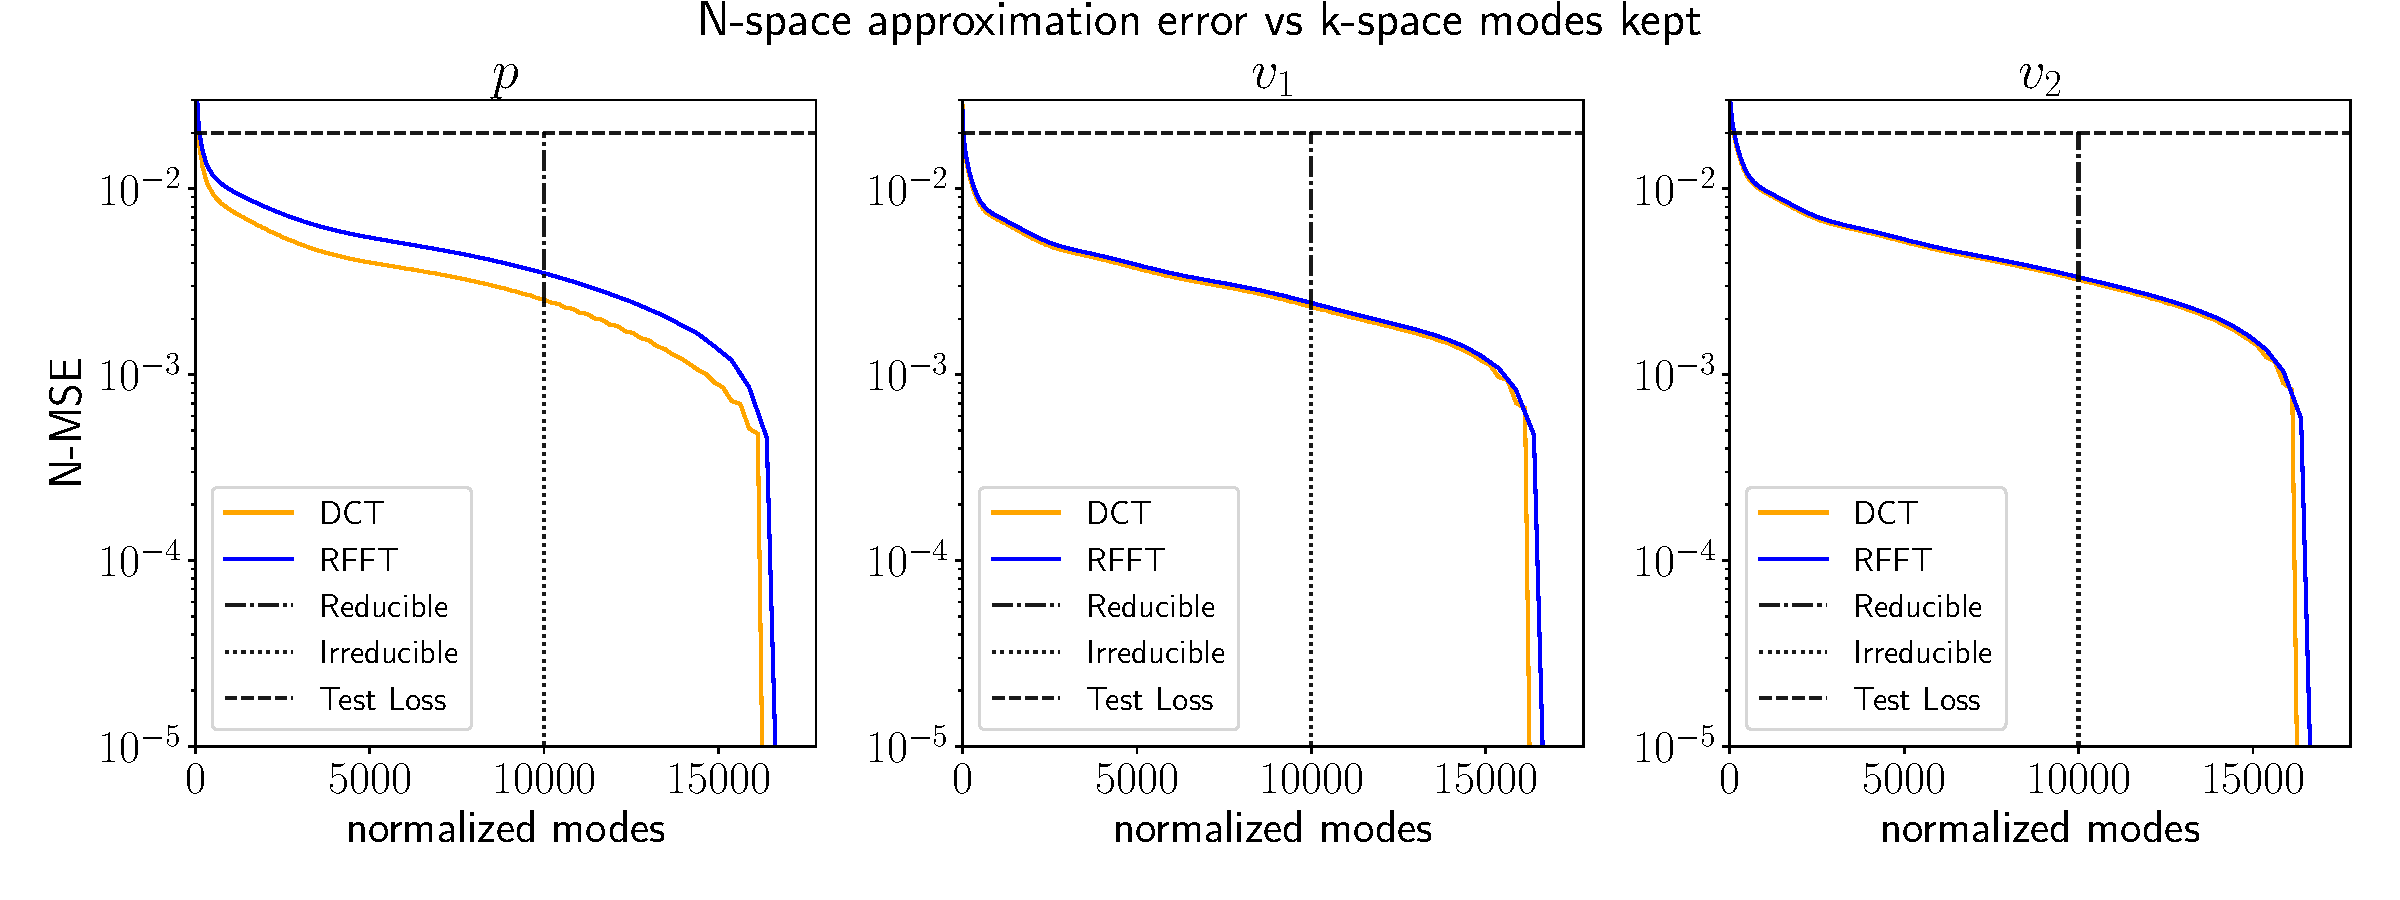
\includegraphics[width=1\linewidth]{figures/dfp_spectrum_approx.pdf}
    % \vspace{-3mm}
    \vspace{-8mm}
    \caption{\small Average approximation error (N-MSE) due to truncation in k-space at different number of elements $m$ for the \textit{flow around airfoils} dataset. In blue, the real FFT k-space, in orange the regular DCT k-space. On the x-axis, the normalized cost for a number of modes $m$: for DCTs, since the k-space is real, truncation at $m$ modes requires $m^2$ floats, for real FFTs with complex k-space and conjugacy the cost in floats is $4m^2$. The vertical line indicates the budget used for \ourmethod{} used in this task ($m=100$), while the horizontal line is the test N-MSE achieved.} 
    \label{fig:dfp-approx-decay}
    
\end{figure*}



\paragraph{Hyperparameter tuning}
%
This is an example of a dataset where the k-space is full due to discontinuity in the solution given by the airfoil mask.

We use the training and validation sets to inspect the k-space and set $m$ to $100$ for the irreducible loss term to be sufficiently small as shown in \cref{fig:dfp-approx-decay}. We swept over $m$ for FNOs and found larger than $24$ to perform worse, likely due to k-space convolution being sufficient to capture higher frequency components. We observe DFPNets with larger channel exponents perform worse due to overfitting. 

\paragraph{Further comments}

A sample of predictions is given in \cref{fig:dfp-predictions-big}. \cref{fig:dfp-nspace-kspace} shows the n-space and corresponding DCT k-space of a data point. As can be observed, the k-space is structured but full due to the discontinuity caused by the airfoil mask. \cref{fig:dfp-approx-decay} shows the approximation error on solution fields due to truncation in k-space at different $m$. In this task, the DCT is more efficient, given a budget of modes to keep, as it yields lower errors. This error provides a theoretical lower bound for the predictive error achievable by a \ourmethod{} model with a given budget, reachable only if the \ourmethod{} predicts the first $m$ modes perfectly.

The vertical line indicates the budget used for the main text \ourmethod{} experiments ($m=100$), and the horizontal one the test N-MSE achieved. Various segments of the vertical line indicate reducible and irreducible components of the loss as discussed in \cref{subsec:inverse}. The theoretical limit at $m=100$ is well below what has been empirically achieved by \ourmethod{} and other models. Indeed, the irreducible loss is an order of magnitude smaller than what the best model (including non-reduced-order variants) achieves on the task. 


\subsection{Turbulent Smoke}\label{asec:exp_sf}
%
\paragraph{Dataset}


We employ for this experiment the ScalarFlow dataset introduced in \citep{eckert2019scalarflow} which is available online under the Creative Commons license CC-BY-NC-SA 4.0\footnote{ScalarFlow dataset download: \href{https://ge.in.tum.de/publications/2019-scalarflow-eckert/}{https://ge.in.tum.de/publications/2019-scalarflow-eckert/}}. \cite{eckert2019scalarflow} created an environment for controlling the release of smoke plumes: a fog machine generated fog inside of a container; the fog was then heated up by a heating cable and a valve controlled its release. Data was captured via multiple calibrated cameras in high resolution at $60$ fps (frames per second) for $150$ frames. 

\begin{figure*}[h!]
    \centering
    % \vspace{-10mm}
    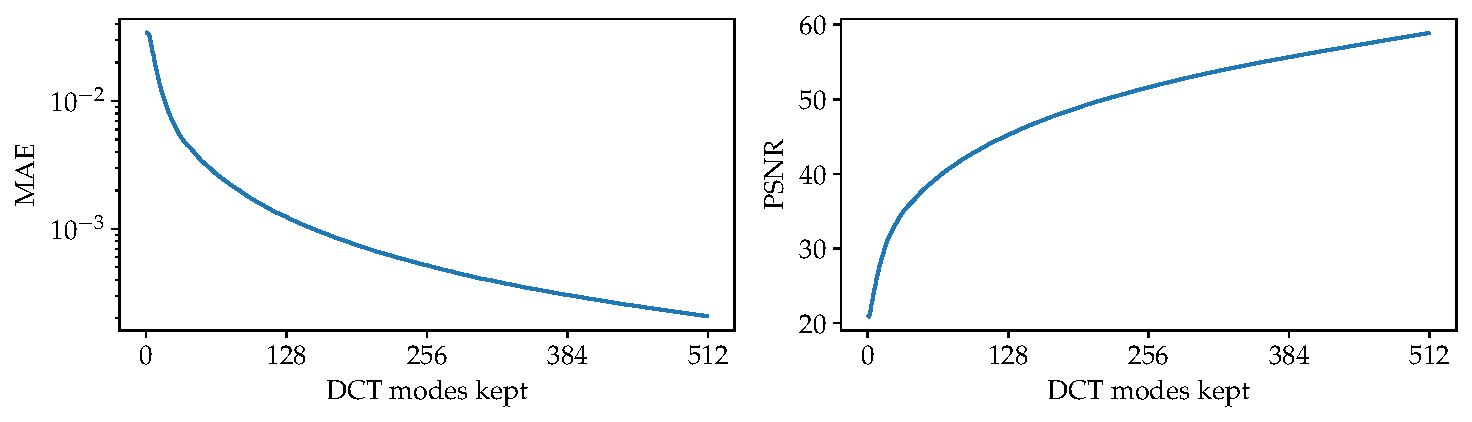
\includegraphics[width=0.8\linewidth]{figures/scalarflow_error_vs_dct_modes.pdf}
    % \vspace{-3mm}
    \caption{\small ScalarFlow dataset: reconstruction error versus number of kept DCT modes.}
    \label{fig:scalarflow-modes-mae-psnr}
    \vspace{-3mm}
\end{figure*}

The dataset contains 3D reconstructions of the smoke plumes and 2D input and rendered images: input images are used by \cite{eckert2019scalarflow} to solve an optimization problem in which the goal is to generate a 3D reconstruction that minimizes the difference between input and rendered images. 2D input images are obtained directly from raw data on which only post-processing is applied by \citep{eckert2019scalarflow} in the form of gray scaling and denoising: these are saved in compressed $\tt numpy$ \citep{harris2020array} arrays named $\tt imgsTarget\_000xxx.npz$. Each resulting frame comprises $5$ different camera views $600\times1062$ in size. Since we want to use \ourmethod{} on high-resolution experimental data, we directly utilize the central camera view of these input images in our learning task without any further downsampling or data processing. Similarly to \citep{lienen2022learning}, we divide the  $104$ recordings into the first $64$ for training and use the remaining $20$ for validation and $20$ for testing. 

Data is normalized to the $[0,1]$ range based on training dataset statistics.
%

\paragraph{Hyperparameter selection and tuning}
We performed a search on the most representative hyperparameters. One of the most important hyperparameters to choose from is the number of DCT modes to keep, i.e. first $m$ elements in $k$-space. We note that for simplicity as well as for compatibility with the UNet inside of \ourmethod{+}, we consider a  \textit{square} mode pruning, i.e. we keep the same number of frequencies on both height and width of the image and refer to the modes kept in both dimensions as $m$. \cref{fig:scalarflow-modes-visualization} and \cref{fig:scalarflow-modes-mae-psnr} show trends of DCT modes in terms of errors and visual quality: while the first modes $m$ contribute the most to the quality of the representation in $n$-space, the last elements contribute only to high-frequency details whose effect is minor on the overall reconstruction. Thus, we set \ourmethod{+} to $m=224$ and consequently \ourmethod{} to $m=512$ to have comparable model sizes. We set $m=48$ for FNO due to memory and model size limitations, noting that its residual connections effectively enlarge the training spectrum to all possible frequencies as shown in \cref{fig:scalarflow-comparison-raw}. Similarly to other experiments (B2), we observe raising $m$ in FNO to not significantly improve predictive error, even when the additional k-space elements would include a larger portion of the dataset.

\begin{figure*}[h!]
    \centering
    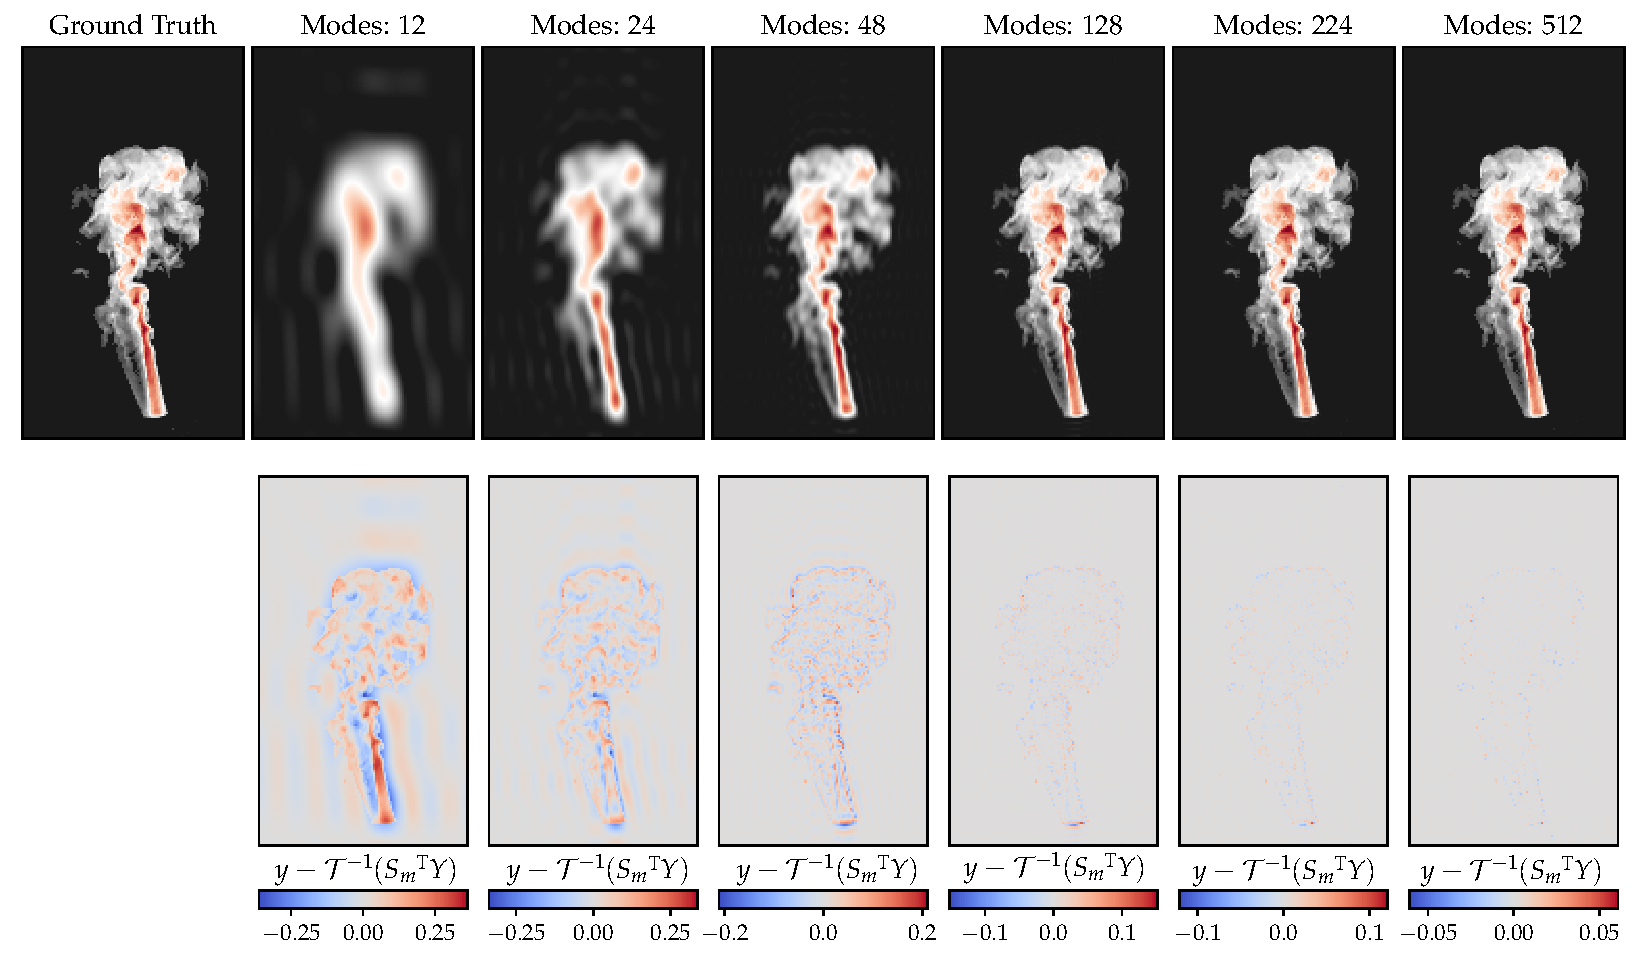
\includegraphics[width=0.95\linewidth]{figures/scalarflow_modes_error_t.pdf}
    % \vspace{-3mm}
    \captionof{figure}{\small \textbf{[Top]} Visual comparison of ScalarFlow frames with changing number of DCT modes kept (i.e. first $m$ elements) .
    \textbf{[Bottom]} Error between the ground truth frame $y$ and its inverse transformation after mode pruning from $k$-space back to $n$-space. As expected, the first few k-space elements are crucial to minimizing reconstruction errors, with higher frequency components contributing minimally.}
\label{fig:scalarflow-modes-visualization}
\end{figure*}

We also experiment with different iterative rollout update strategies as in \citep{pfaff2020learning}. We consider the time step $\Delta t$ to be unitary, i.e. $\Delta t = 1$, given that the training frames are sampled consistently at 60 fps. We call $0$-order integration an update of the type: $x_{t+1} = h_\theta(x_t; x_{t-1}, \dots, x_{t-H})$ in which $h_\theta$ denotes a learned model which takes as inputs the current state $x_t$ and optionally a history of size $H$ of past states $x_{t-1}, \dots, x_{t-H}$ and directly predicts the next state $x_{t+1}$. A $1$-order integrator performs the following update: $x_{t+1} = x_t + h_\theta(x_t; \cdot)$, in which the model predicts the state update, i.e. the \textit{velocity}, similarly to an Euler step. A $2$-order integrator, also known as basic Störmer–-Verlet \citep{verlet1967computer} can be written as following: $x_{t+1} = 2x_t - x_{t-1} + h_\theta(x_t; \cdot)$; the model $h_\theta$ predicts the \textit{acceleration} of the system. We empirically found the zero-order integration to be more prone to generating artifacts with slower convergence, which may be because the model has to directly predict the next step with no "help" from the current step information. We found models trained with first-order integrators to have lower predictive errors than those trained with second-order ones, and we thus use it in all the experiments. As for the history size, we selected $H=1$ since it provided noticeable benefits compared to $H=0$, in which the model has no way of knowing previous states and thus inferring velocities. Larger history sizes did not seem to provide any improvements and only made the models larger as also noted in \citep{pfaff2020learning}.  

\begin{figure}
    \centering
    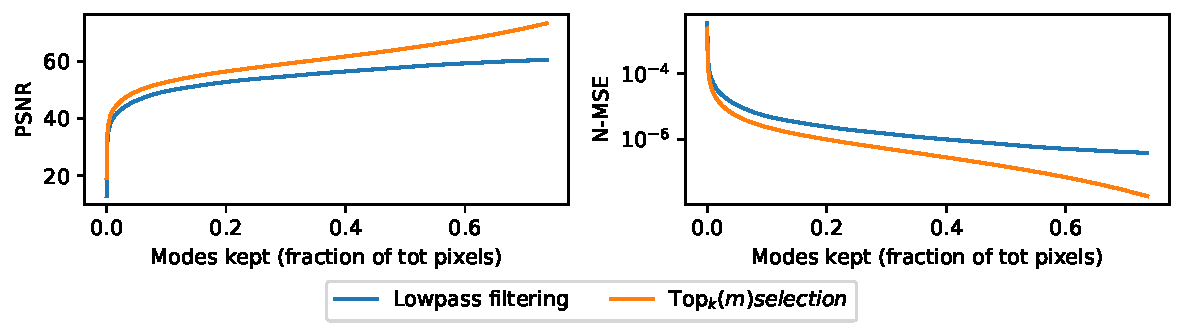
\includegraphics[width=\linewidth]{figures/scalarflow_topk.pdf}
    \vspace{-5mm}

    \caption{\footnotesize Reconstruction errors in pixel space of low-pass filtering of the lowest $m$ frequency modes vs ${\tt top}_k(m)$ selection on a single frame of ScalarFlow.}
    \vspace{-5mm}
    \label{fig:sflow_topk}
\end{figure}

\paragraph{Mode selection} We further show in \cref{fig:sflow_topk} the effect of simple low-pass filtering of lowest $m$ frequency modes and ${\tt top}_k(m)$ mode selection in pixel space reconstruction (as a fraction of total pixes, i.e., $600 \times 1062$). The latter achieves better reconstruction results with the same number of parameters.




% Trick for the configs
% If this environment is on the first element of a page, it breaks - make sure this doesnt happen
% \pagebreak % remove if not needed!!
\pagebreak
\paragraph{Models and training}

All models share the configuration for training:

\begin{listing}[H]
\begin{mintedbox}{yaml}
datamodule: 
    ntrain: 64
    nval: 20
    ntest: 20
    batch_size: 1
    history_size: 1
    target_steps_train: 3
    target_steps_val_test: 10
train:
    optimizer: 
        type: AdamW
        learning_rate: 1e-3
        weight_decay: 1e-4
    scheduler:
        type: CosineAnnealingWarmRestarts
        T_0: 32
        step_size: 1
        scheduler_interval: step
loss_fn: RelativeL2Loss
\end{mintedbox}
\vspace{-6mm}
\end{listing}



Where we used the implementation in $\tt PyTorch$ of the cosine annealing schedule with warm restarts\footnote{We used the scheduler \href{https://pytorch.org/docs/stable/generated/torch.optim.lr_scheduler.CosineAnnealingWarmRestarts.html}{$\tt torch.optim.lr\_scheduler.CosineAnnealingWarmRestarts$} with the number of iterations for the first restart $T\_0 = 32$. All other hyperparameters are the same as in the reference implementation.}.
The FNO architecture comprises a standard stack of FDM layers as discussed in B.1. The k–space UNet in \ourmethod{+} (and in its $\tt vp$ variant) has the same structure as a DFPNet.


\begin{listing}[H]
\begin{minipage}[t]{0.32\textwidth}
\begin{mintedbox}{yaml, title=\config{FNO}}
modes: 48
nlayers: 4
width: 48 \end{mintedbox}
\end{minipage}
%
\begin{minipage}[t]{0.32\textwidth}
\begin{mintedbox}{yaml, title=\config{\ourmethod{}}}
modes: 512
nlayers: 4
width: 8  \end{mintedbox}
\end{minipage}
%
\begin{minipage}[t]{0.32\textwidth}
\begin{mintedbox}{yaml, title=\config{\ourmethod{+}}}
modes: 224
nlayers: 1
width: 4
channel_exponent: 7 \end{mintedbox}
\end{minipage}
\vspace{-6mm}
\end{listing}

where we note that all models employ $\tt GeLU$ \citep{hendrycks2016gaussian} activation functions between inner layers. 


\paragraph{Analysis of results}
\begin{figure*}[h!]
    \centering
    % \vspace{-10mm}
    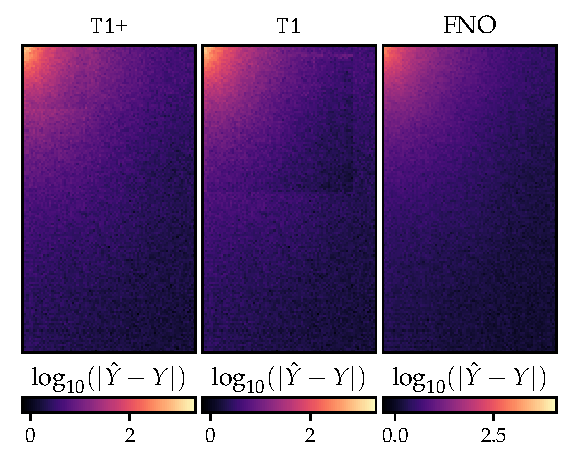
\includegraphics[width=0.4\linewidth]{figures/scalarflow_dct_errors_batch.pdf}
    \vspace{-3.5mm}
    \caption{\small Mean log-absolute values of predictions in $k$-space (DCT-II) of a $20$-elements batch in the test dataset. Although \ourmethod{} is limited to $m=512$ and \ourmethod{+} to $m=224$ $k$-space elements (visible as square "shadows" in the error plots), its predictions are overall more physically accurate in $n$-space.}
    \label{fig:scalarflow-dct-batch-error}
\end{figure*}

\begin{table}[b]
    \caption{Full benchmark on the ScalarFlow dataset over 5 runs with different random seeds. N-MSE refers to 10-step test rollouts. \ourmethod{+vp} generates more stable rollouts while requiring a fraction of FNO's training time.}
    \centering
    \begin{tabular}{c|c c c c }\toprule
        \textbf{Method} & Param (M) & Size (MB) & Time (hrs) & N-MSE ($\times 10^{-1}$) \\
        \toprule
        FNO & 84.9 & 339 & 32.4 & 2.32 $\pm$ 0.02 \\ 
        \ourmethod{} & 83.9 & 335 & 8.1 & 2.39 $\pm$ 0.02\\ 
        \ourmethod{+} & 67.8 & 271 & 4.7 & 2.56 $\pm$ 0.16\\
        \ourmethod{+vp} & 67.8 & 271 & 4.7 & 2.28 $\pm$ 0.09\\
        \bottomrule
    \end{tabular}
    % \vspace{-1.4mm}
    \label{tab:scalarflow-large}
% \end{wraptable}
\end{table}



\cref{tab:scalarflow-large} provides a larger version of the table in the main text, including $1$-step mean absolute errors (MAE). We note that while FNO produces smaller errors in one-step predictions, it quickly accumulates larger errors in extrapolation. \cref{fig:scalarflow-dct-batch-error} shows mean errors in $k$-space of FNO vs \ourmethod{} and \ourmethod{+}. \ourmethod{} models demonstrate smaller overall errors and lower maxima compared to the FNO.

% \begin{wraptable}[0]{r}{\linewidth}
